%% Run LaTeX on this file several times to get Table of Contents,
%% cross-references, and citations.

\documentclass[11pt]{book}
\usepackage{gvv-book}
\usepackage{gvv}
\usepackage[sectionbib,authoryear]{natbib}% for name-date citation comment the below line
\setcounter{secnumdepth}{3}
\setcounter{tocdepth}{2}

\makeindex

\begin{document}

\frontmatter

\booktitle{GEOMETRY}

\subtitle{Through Algebra}

\AuAff{Chakali Suresh}

\titlepage

\tableofcontents

\setcounter{page}{1}

\mainmatter

\chapter{Triangle}
Consider a triangle with vertices
\begin{align}
\vec{A} = \myvec{0 \\ -5},\,
\vec{B} = \myvec{-2 \\ -4},\,
\vec{C} = \myvec{-5 \\ -4}
\end{align}

\section{Altitude}
\begin{enumerate}[label=\thesection.\arabic*.,ref=\thesection.\theenumi]
\numberwithin{equation}{enumi}

%Question 1.3.1: 
\item $\vec{D}_1$ is a point on $BC$ such that
		\begin{align}
			AD_1 \perp BC
		\end{align}
		and $AD_1$ is defined to be the altitude. 
		Find the normal vector of $AD_1$.\\
\solution\\
Given
\begin{align}
\vec{A} = \myvec{0 \\ -5},\\
\vec{B} = \myvec{-2 \\ -4},\\
\vec{C} = \myvec{-5 \\ -4}
\end{align}
Normal vector of $AD1$ is orthogonal to $AD1$ and hence parallel to $BC$.Direction vector $\vec{m_{BC}}$\\
\begin{align}
	&= \vec{C} - \vec{B}\\
        &= \myvec{-5 \\ -4} - \myvec{-2 \\ -4}\\
        &= \myvec{-3 \\ 0}\\
        \text{Normal vector of } \vec{AD1} &= \myvec{-3 \\ 0}
\end{align}

%Question 1.3.2:
\item Find the equation of $AD_1$. \\
\solution\\
The normal vector of
\begin{align}
\implies \vec{n} &= \myvec{-3 \\ 0}
\end{align}
The equation of $AD_1$ is
\begin{align}
 \vec{n}^{\top}(\vec{x-A}) &= 0 \\
 \vec{n}^{\top}(\vec{x}) &= \vec{n}^{\top}(\vec{A})\\
\implies \myvec{-3 & 0}\vec{x} &= \myvec{-3 & 0}\myvec{0 \\ -5}\\
\myvec{0 & 3}\vec{x} &= 0
\end{align}
\begin{figure}[H]
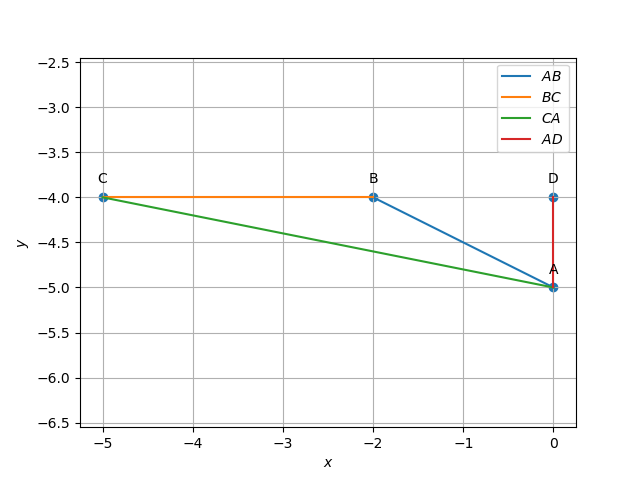
\includegraphics[width=\columnwidth]{/sdcard/Documents/figs/AD}
\caption{Altitude $AD_1$}
\label{fig:Line AD}
\end{figure}

%Question 1.3.3:
	\item Find the equations of the altitudes $BE_1$ and $CF_1$ to the sides $AC$ and $AB$ respectively.\\
 \solution\\
The normal equation of $CF_1$ is 
\begin{align}
\vec{n} &= \myvec{-2\\1} \\
\vec{n}^{\top}\brak{\vec{x}-\vec{C}} &= 0 \\
\vec{n}^{\top}\brak{\vec{x}} &= \vec{n}^{\top}\brak {\vec{C}} \\
\implies \myvec{-2 & 1}{\vec{x}} &= \myvec{-2 & 1} \myvec{-5 \\ -4}  \\
	\implies \myvec{-2 & 1}\vec{x} &= 6
\end{align}
The normal equation of $BE_1$ is 
\begin{align}
\vec{n} &= \myvec{-5 \\ 1}\\
\vec{n}^{\top}\brak{\vec{x}-\vec{B}} &= 0 \\
\vec{n}^{\top}\brak{\vec{x}} &= \vec{n}^{\top}\brak {\vec{B}}\\
	\implies \myvec{-5 & 1}\vec{x} &= \myvec{-5 & 1} \myvec{-2 \\ -4}\\
	\implies \myvec{-5 & 1}\vec{x} &= 6
\end{align}
\begin{figure}[H]
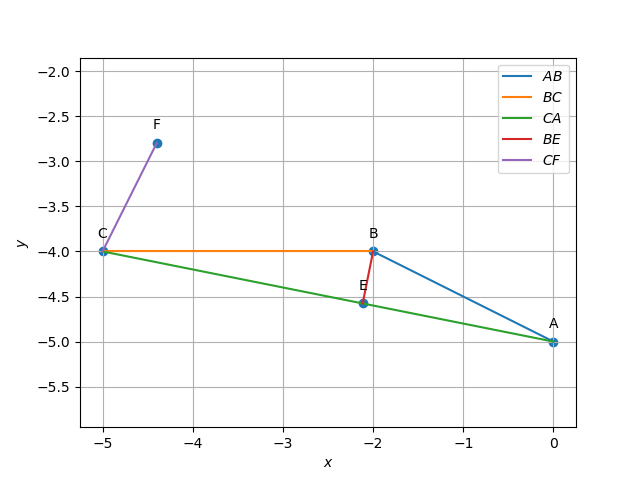
\includegraphics[width=\columnwidth]{/sdcard/Documents/figs/BE_CF}
\caption{Altitudes $BE_1$ and $CF_1$ }
\label{fig:Line BE and CF}
\end{figure}

%Question 1.3.4:
	\item Find the intersection $\vec{H}$ of $BE_1$ and $CF_1$.\\
\solution\\
 Equation of $BE_1$
 \begin{align}
     \myvec{-5 & 1}\vec{x} &= 6
 \end{align}
  Equation of $CF_1$
 \begin{align}
    \myvec{-2 & 1}\vec{x} &= 6
 \end{align}
Therefore, we need to solve the following equation to get $\vec{H}$:
\begin{align}
        \myvec{-5 & 1\\-2 & 1} \vec{x} &= \myvec{6 \\ 6}
\end{align}
Solving the above equation by Gauss-Jordan method
\begin{align}
        \myvec{-5 & 1 & 6\\-2 & 1 & 6}
	 \xleftrightarrow[]{R_1 \leftarrow \frac{R_1}{-5}}
        \myvec{1 & \frac{-1}{5} & \frac{-6}{5}\\-2 & 1 & 6}\\
	 \xleftrightarrow[]{R_2 \leftarrow R_2 + 2R_1}
        \myvec{1 & \frac{-1}{5} & \frac{-6}{5}\\0 & \frac{3}{5} & \frac{18}{5}}\\
	 \xleftrightarrow[]{R_2 \leftarrow \frac{5R_2}{3}}
        \myvec{1 & \frac{-1}{5} & \frac{-6}{5}\\0 & 1 & 6}\\
        	 \xleftrightarrow[]{R_1 \leftarrow R_1 + \frac{R_2}{5}}
                  \myvec{1 & 0 & 0\\0 & 1 & 6}
\end{align}
Therefore point of intersection $\vec{H}$ is
\begin{align}
	&= \myvec{0 \\ 6}
\end{align}
\begin{figure}[H]
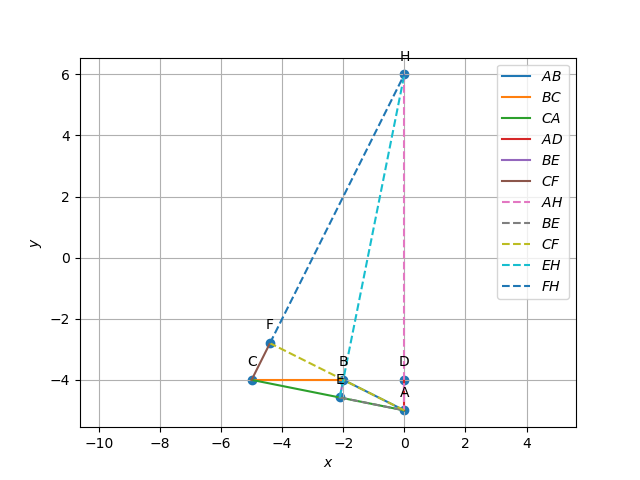
\includegraphics[width=\columnwidth]{/sdcard/Documents/figs/Intersection}
	\caption{Intersection point $\vec{H}$ of altitudes $BE_1$ and $CF_1$}
\label{fig:Interction point}
\end{figure}

%Question 1.3.5:
\item Verify that 
		\begin{align}
			\brak{\vec{A}-\vec{H}}^{\top}\brak{\vec{B}-\vec{C}} = 0
		\end{align}\\
  \solution\\
Given
\begin{align}
            \vec{A} &= \myvec{0 \\ -5}, \vec{B} = \myvec{-2 \\ -4}\\
            \vec{C} &= \myvec{-5 \\ -4}, \vec{H} = \myvec{0 \\ 6}
\end{align}
To solve the equation
\begin{align}
\vec{A}-\vec{H} &= \myvec{0 \\ -5} - \myvec{0 \\ 6}\\
                &= \myvec{0 \\ -11}\\
\vec{B}-\vec{C} &= \myvec{-2 \\ -4} - \myvec{-5 \\ -4}\\
                &= \myvec{3 \\ 0}\\
	\implies \brak{\vec{A}-\vec{H}}^{\top}\brak{\vec{B}-\vec{C}} &= \myvec{0 & -11} - \myvec{3 \\ 0}\\
                &= 0
\end{align}
\begin{figure}[H]
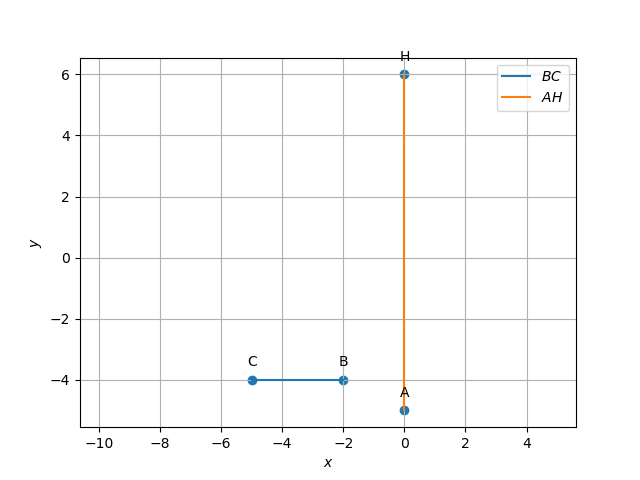
\includegraphics[width=\columnwidth]{/sdcard/Documents/figs/AH}
\caption{Plot of points $A, B, C$ and $H$}
\label{fig1:Points}
\end{figure}

\latexprintindex

\end{enumerate}
\end{document}
